\section{Introduzione}

Il seguente documento vuole fornire una guida sull'utilizzo del prodotto ENGaming, mostrando le schermate disponibili ed interagibili da parte dell'utente che usufruisce dell'applicazione.

\subsection{ENGaming}

Uno dei mercati dove opera Euronovate è quello dei device di firma grafometrica dotati di monitor da 10 pollici multi-touch.\\ 
ENGaming punta al mondo dei multimedia e vuole permette l'utilizzo del device di firma ENSign 11 per l'intrattenimento videoludico.\\ 
L'obiettivo è realizzare un applicativo che permetta di selezionare un videogioco da una lista di giochi pre-configurata e avviarlo assieme ad un controller virtuale.\footnote[1]{\href{https://www.assindustriavenetocentro.it/2023/stage-it}{Stage IT 2023}, azienda ESignWorld}

\subsection{Device utilizzato}

Come citato nella sezione precedente, il device che verrà utilizzato è l'ENSign 11, un dispositivo utilizzato principalmente per la digitalizzazione delle firme a mano, per firme biometriche e come schermo di presentazione multi-touch.\\
Direttamente connesso al computer tramite porta USB, l'ENSign 11 è un device molto compatto con grande stabilità, livelli di sicurezza alti e dotato di un elegante design.\footnote[2]{\href{https://www.euronovategroup.com/solutions/product-map/ensign-11-ensign-nfc-hardware}{ENSign 11}, descrizione prodotto}

\newpage
\section{Requisiti di sistema}
Per poter utilizzare l'applicazione, è necessario avere a disposizione:
\begin{itemize}
    \item un PC con installato il driver DisplayLink\footnote[3]{\href{https://www.synaptics.com/products/displaylink-graphics}{DisplayLink}} e uno dei seguenti sistemi operativi: \begin{itemize}
    \item Windows 11 (non necessario installare il driver citato in precedenza, in quanto già presente).
    \item MacOS Ventura.
    \end{itemize}
    \item un ENSign11 da collegare a suddetto PC.
\end{itemize}
L'applicazione può funzionare anche con precedenti versioni di Windows e MacOS, ma non essendo stati effettuati test in merito non se ne garantisce il supporto.\\
I sistemi operativi con kernel Linux non sono attualmente supportati, ma se ne prevede il supporto in futuro.\\
L'utilizzo di un device diverso dall'ENSign11 è sconsigliato e non se ne garantisce il supporto.
\section{Installazione dell'applicazione}
Per poter utilizzare l'applicazione, è necessario installarla utilizzando l'apposito file.
Dopo qualche minuto, si aprirà l'applicazione sull'ENSign11 collegato al dispositivo.
\newpage
\section{Schermata iniziale}
Una volta avviata l'applicazione, si avrà di fronte la schermata iniziale dell'applicazione, che comprende:
\begin{itemize}
    \item Il nome dell'applicazione, ovvero ENGaming.
    \item L'elenco dei giochi disponibili, sotto forma di icone.
    \item Un'icona per visualizzare i record effettuati.
    \item Un'icona per uscire dall'applicazione.
\end{itemize}
\begin{figure}[h]
    \centering
    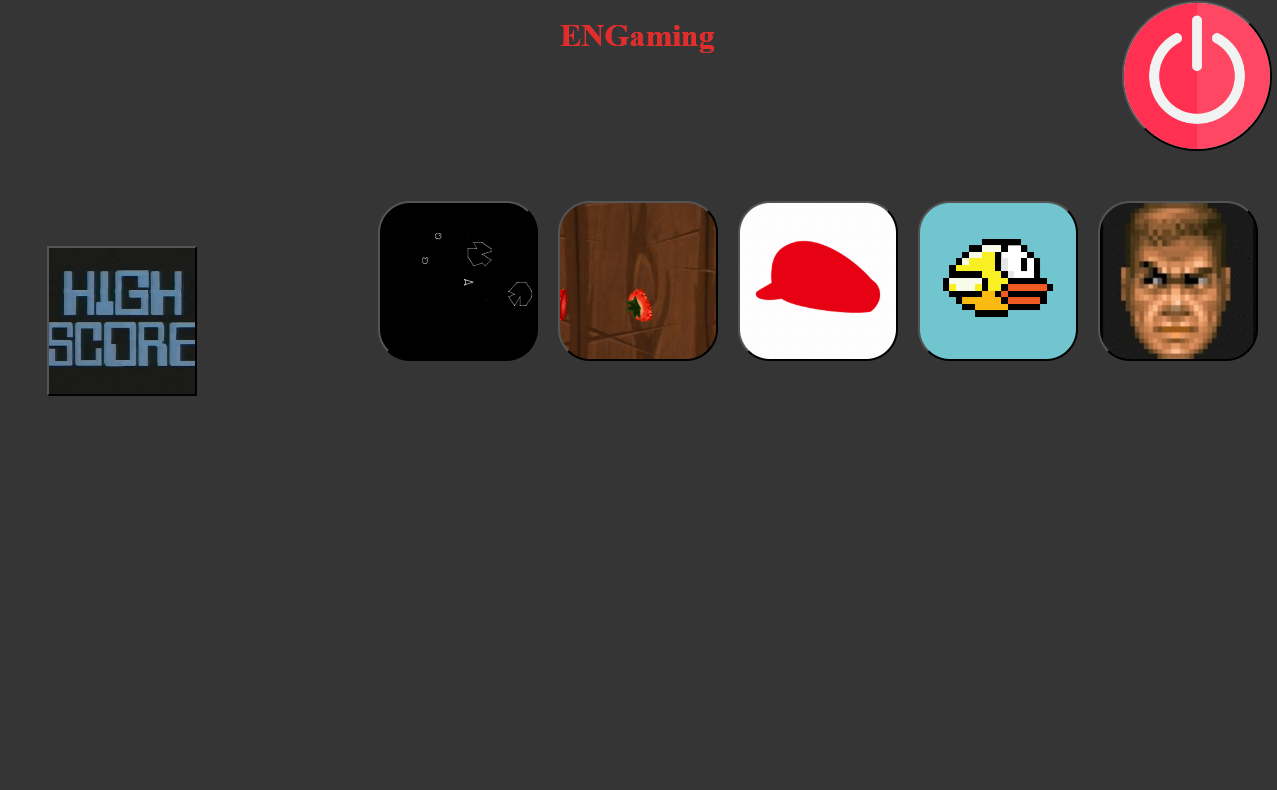
\includegraphics[width=340pt]{schermataIniziale.png}
    \caption{Schermata iniziale di ENGaming}
    \label{fig:schermataIniziale}
\end{figure}
\newpage
\section{Visualizzazione record}
Premendo dalla schermata iniziale l'apposita icona, si passa alla pagina di visualizzazione dei record.
\subsection{Lista dei record globali}
La prima lista di record visualizzabile è la lista dei record globali, dove ogni record fornisce informazioni su:
\begin{itemize}
    \item l'utente che ha effettuato il record
    \item il punteggio totalizzato
    \item la data in cui è stato effettuato il record
    \item il gioco in cui è stato effettuato il record
\end{itemize}
\begin{figure}[h]
    \centering
    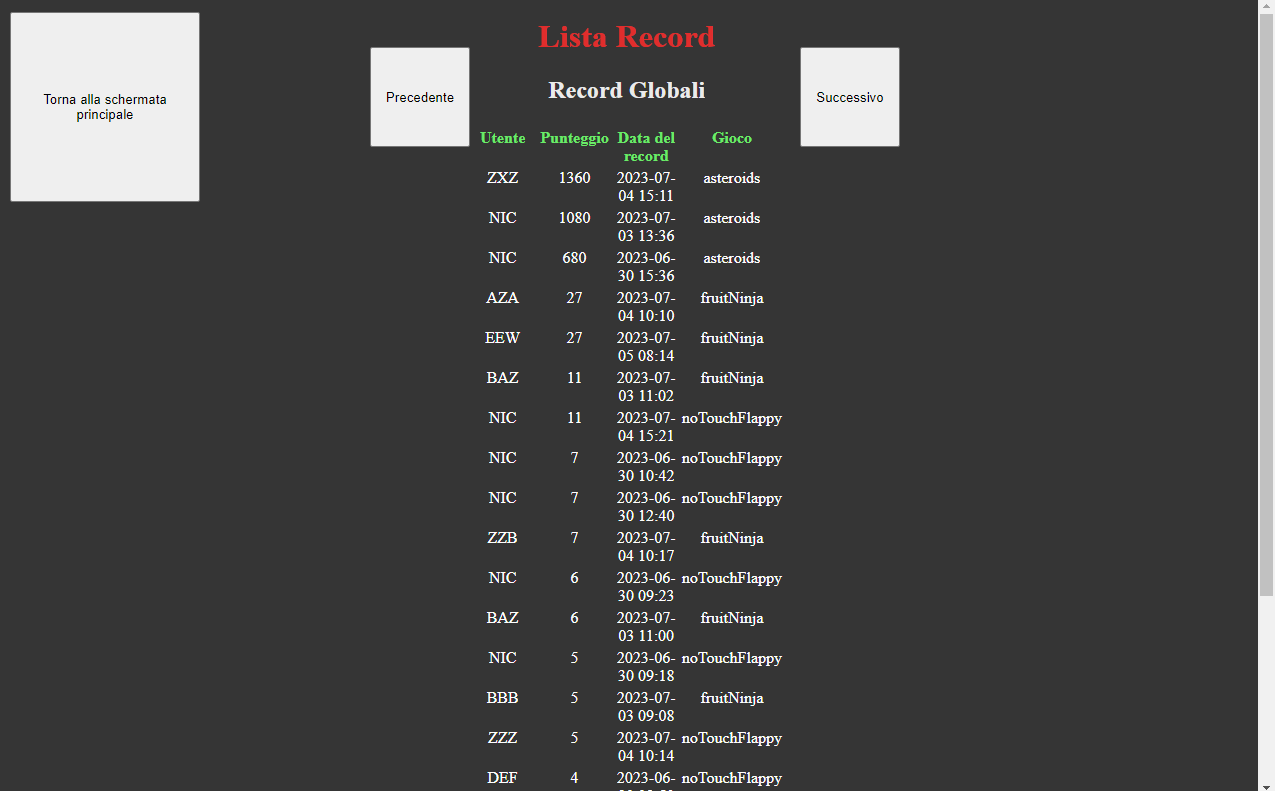
\includegraphics[width=340pt]{schermataRecord.png}
    \caption{Lista dei record globali}
    \label{fig:schermataRecord}
\end{figure}
Premendo sugli appositi pulsanti, viene cambiata la lista di visualizzazione, passando alle liste dei record dei singoli giochi.
Infine, tramite l'apposito pulsante, si ritorna alla schermata iniziale.
\subsection{Lista dei record per un singolo gioco}
Le liste di record per i singoli giochi forniscono le stesse informazioni, ovvero:
\begin{itemize}
    \item l'utente che ha effettuato il record
    \item il punteggio totalizzato
    \item la data in cui è stato effettuato il record
\end{itemize}
Escludendo il gioco, in quanto la lista specifica già il gioco a cui sono associati i record.\\
La prima e l'ultima lista di questo genere, alla pressione degli appositi pulsante, riportano alla lista globale.
\begin{figure}[h]
    \centering
    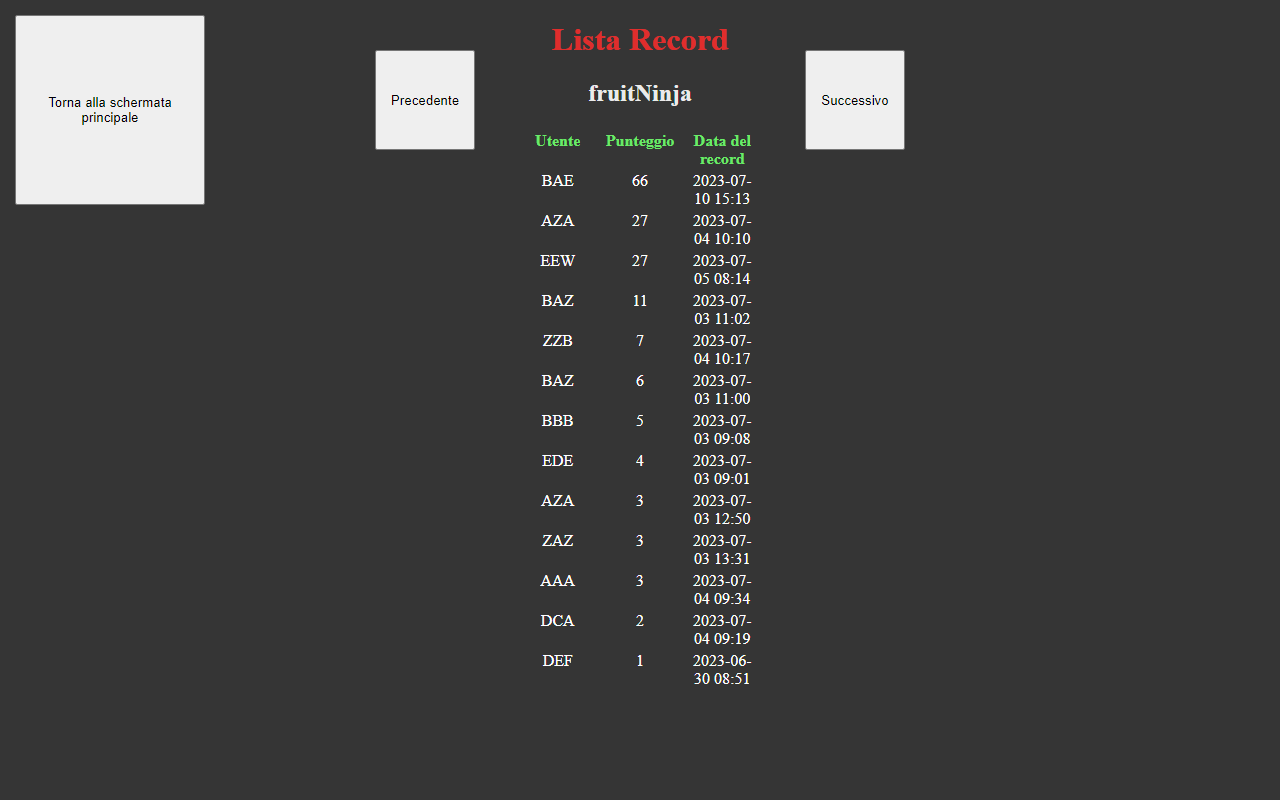
\includegraphics[width=340pt]{schermataRecordSingoloGioco.png}
    \caption{Esempio di lista per un singolo gioco}
    \label{fig:schermataRecordSingoloGioco}
\end{figure}
\newpage
\section{Pagina di un gioco}
Selezionando un'icona di un gioco dal menù principale, si arriva alla pagina di quel gioco.\\
La pagina di un gioco contiene le seguenti informazioni:
\begin{itemize}
    \item il nome del gioco.
    \item il genere del gioco.
    \item il tipo di input, ovvero se viene utilizzato il controller o il touch/digitalizer.
    \item la descrizione del gioco.
    \item L'elenco degli input, o delle gesture, che il gioco ha.
\end{itemize}
Inoltre, da questa pagina si può scegliere se avviare il gioco oppure tornare al menù principale.
\begin{figure}[h]
    \centering
    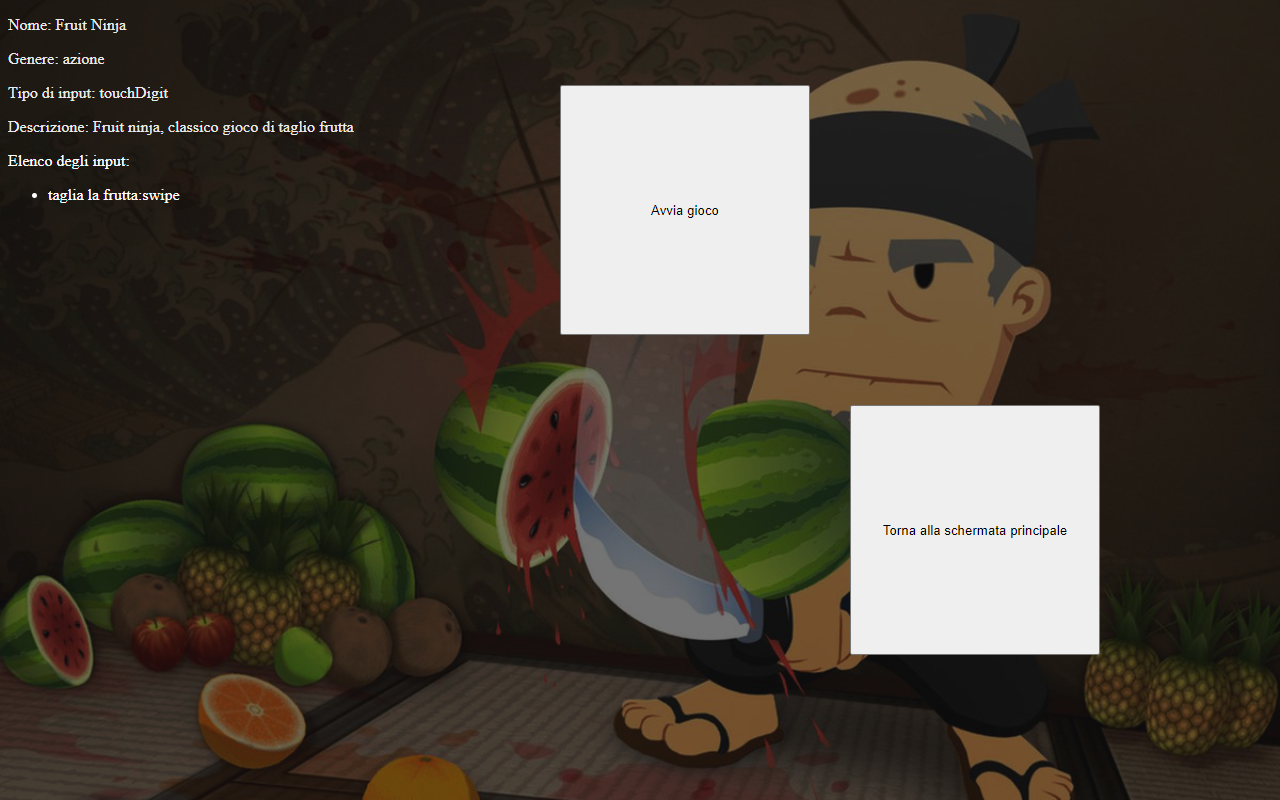
\includegraphics[width=340pt]{schermataPaginaGioco.png}
    \caption{Esempio di pagina di un gioco}
    \label{fig:schermataPaginaGioco}
\end{figure}
\newpage
\section{Avvio di un gioco}
Scegliendo di avviare un gioco dalla propria pagina, si parte dalla visualizzazione di una pagina di caricamento. Si passa successivamente alla schermata di gioco, che varia a seconda della tipologia. Il gioco si conclude passando dalla pagina di pausa.
\subsection{Pagina di caricamento}
La pagina di caricamento informa semplicemente che il caricamento è in corso. Ciò permette al sistema di caricare i file necessari ai giochi e impedisce comportamenti indesiderati.\\
Il tempo di visualizzazione di questa pagina è fissato a 4 secondi.
\begin{figure}[h]
    \centering
    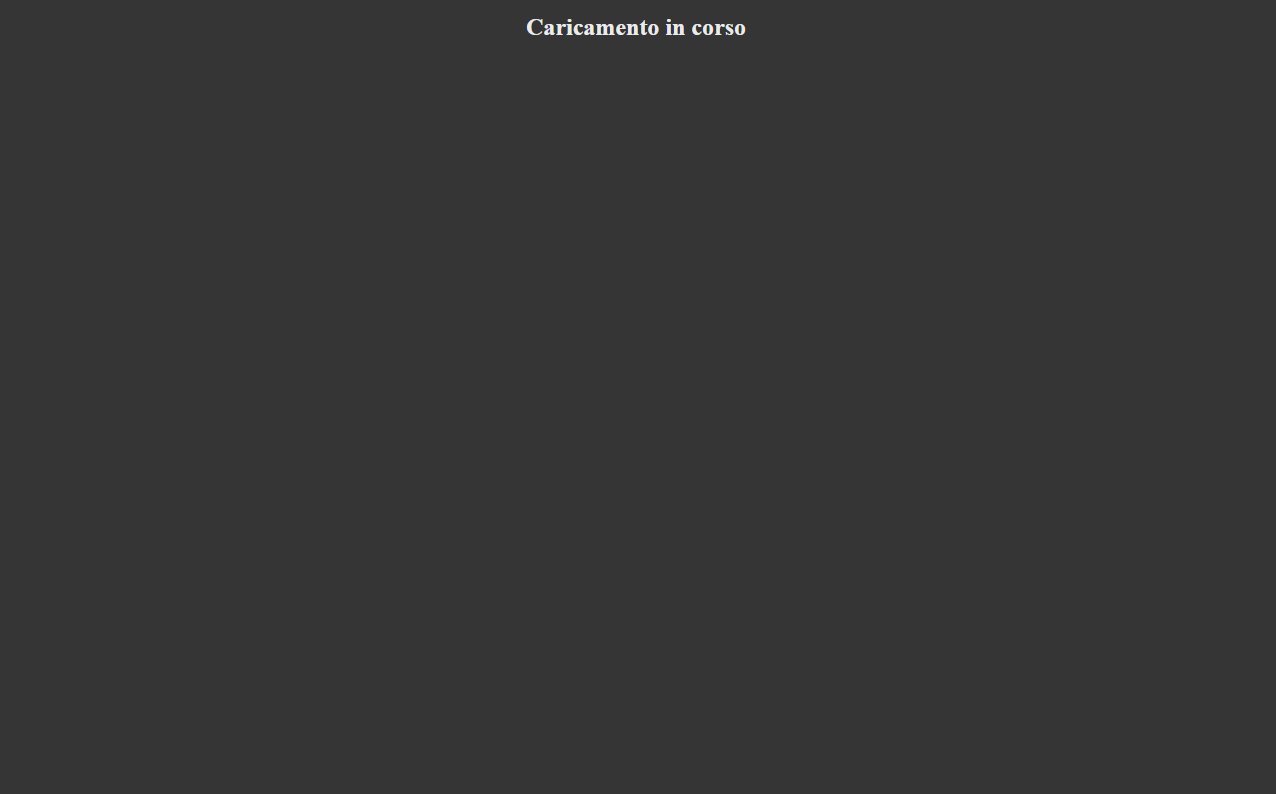
\includegraphics[width=340pt]{schermataCaricamento.png}
    \caption{Schermata di caricamento}
    \label{fig:schermataCaricamento}
\end{figure}
\\Dopo i 4 secondi, si viene reindirizzati alla schermata di gioco prevista, a seconda del gioco stesso.
\newpage
\subsection{Schermata di gioco-controller}
Nel caso di un gioco che richieda l'uso del controller, si viene reindirizzati a questa schermata.\\
La schermata è composta dal gioco stesso e dal controller. Il controller, partendo dalla struttura di default (ovvero 4 tasti direzionali, 4 tasti di azione e il tasto di pausa), viene configurato in base agli input richiesti dal gioco, non mostrando (duqnue, bloccando l'interazione) i pulsanti non necessari.
\begin{figure}[h]
    \centering
    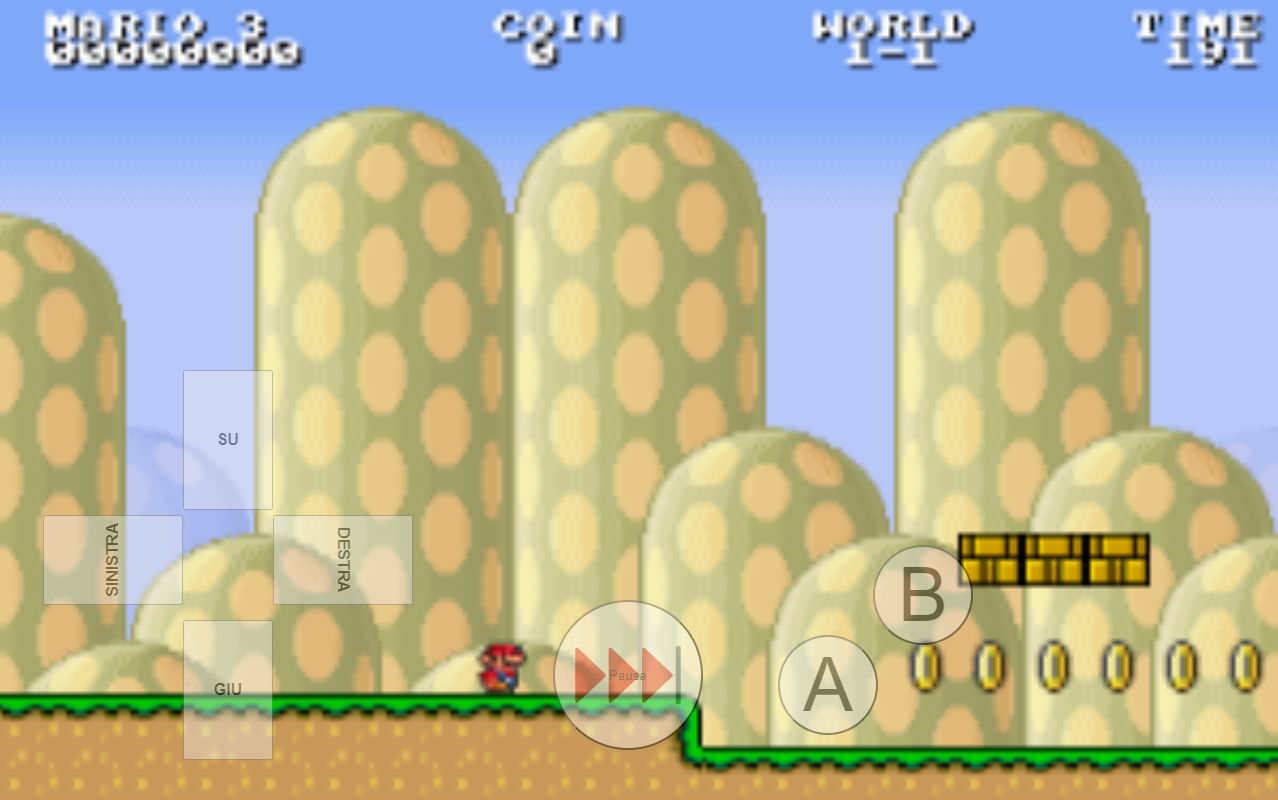
\includegraphics[width=340pt]{schermataGiocoController.png}
    \caption{Esempio di schermata per un gioco con il controller}
    \label{fig:schermataGiocoController}
\end{figure}
\newpage
\subsection{Schermata di gioco-touch/digitalizer}
Nel caso di un gioco che richieda l'uso del touch o del digitalizer, si viene reindirizzati a questa schermata.\\
La schermata è composta dal gioco stesso e dal solo pulsante di pausa, dato che i comandi vengono dati tramite gestures.\\
Il pulsante di pausa è posizionato in modo da intralciare il meno possibile l'utente durante il gioco, al fine di non intaccare l'esperienza d'uso.
\begin{figure}[h]
    \centering
    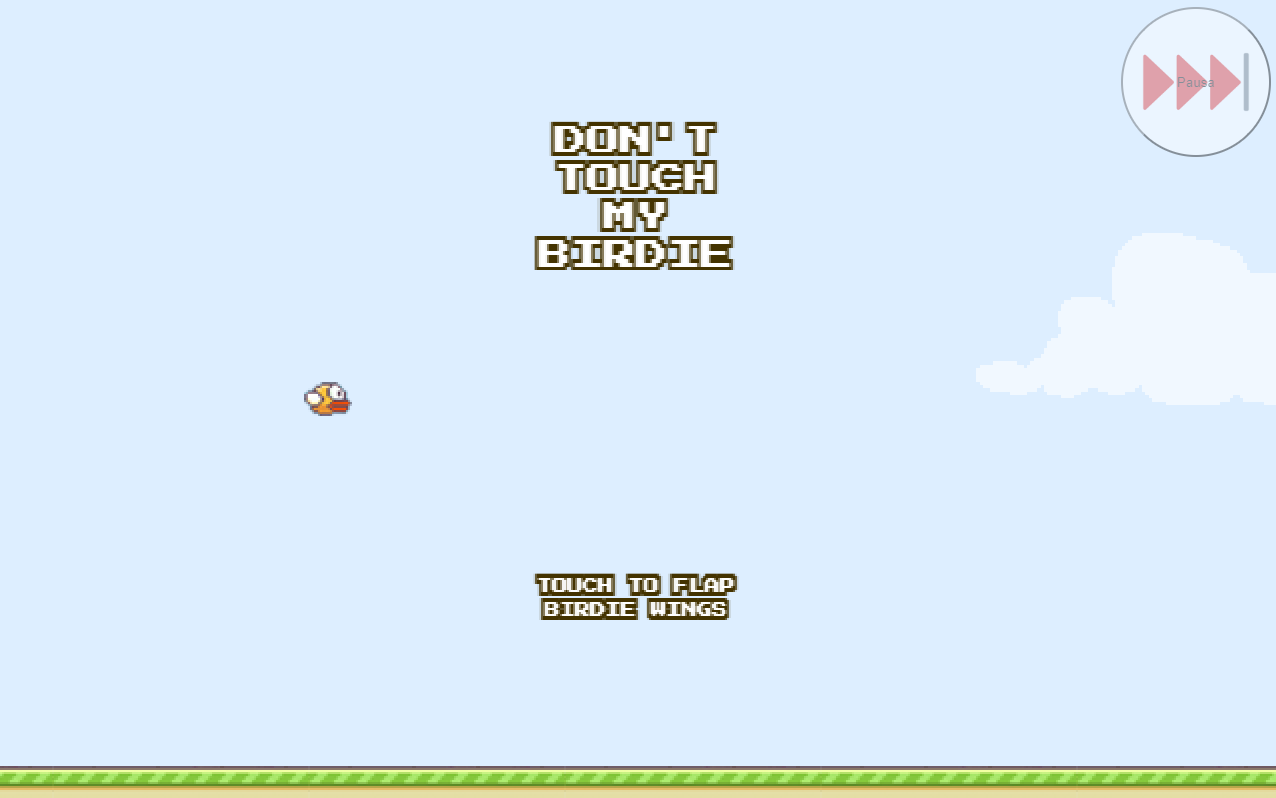
\includegraphics[width=340pt]{schermataGiocoTouchDigit.png}
    \caption{Esempio di schermata per un gioco con il touch/digitalizer}
    \label{fig:schermataGiocoTouchDigit}
\end{figure}
\newpage
\subsection{Pagina di pausa}
Premendo sul pulsante di pausa, si arriva alla schermata apposita.\\
La schermata di pausa, oltre ad informare l'utente dello stato di pausa dell'applicazione, permette di ritornare al gioco attualmente in esecuzione oppure di uscire dal gioco, tornando al menù principale.
\begin{figure}[h]
    \centering
    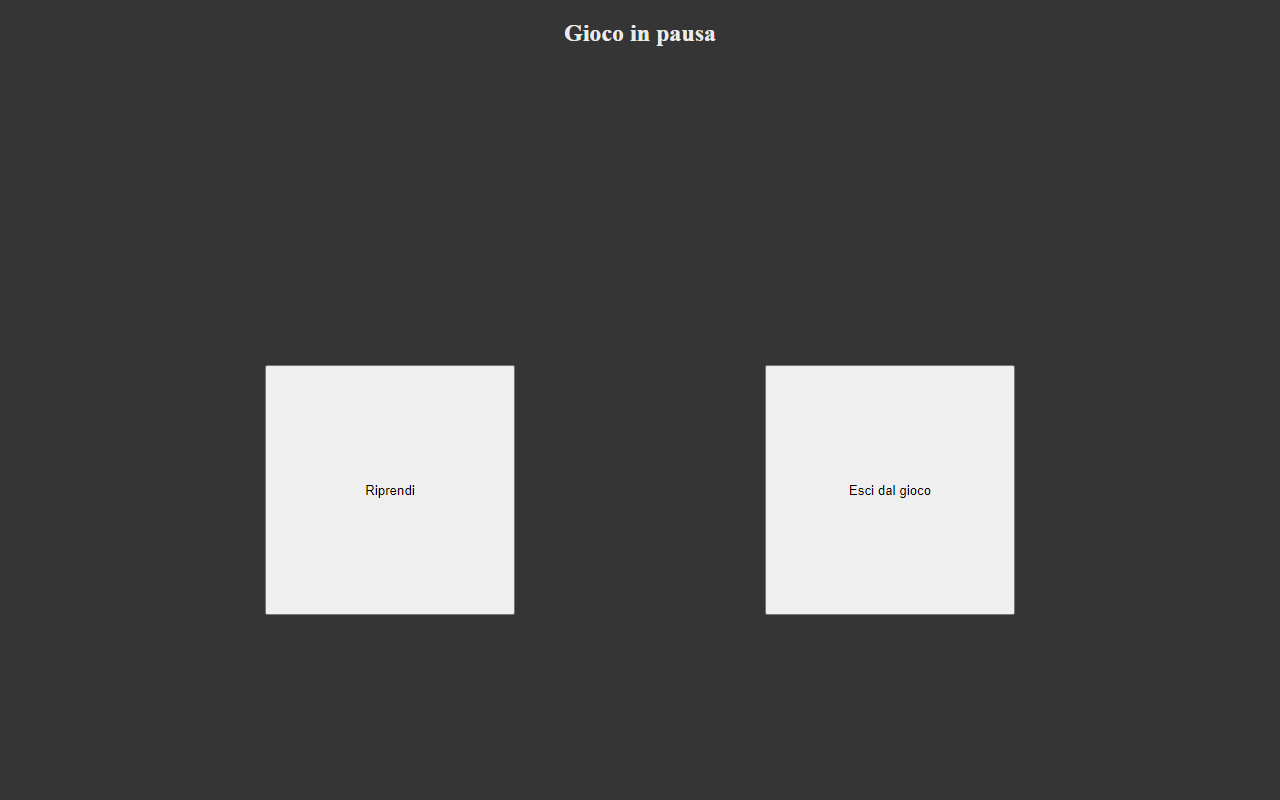
\includegraphics[width=340pt]{schermataPausaGioco.png}
    \caption{Schermata di pausa}
    \label{fig:schermataPausaGioco}
\end{figure}
\subsection{Inattività nei giochi o nella schermata di pausa}
Per quanto accade durante un'eventuale inattività, si rimanda alla sezione di \hyperref[sec:inactivity]{Gestione dell'inattività}
\newpage
\section{Realizzazione di un nuovo record}
Se l'utente, durante la sua sessione di gioco (ovvero da quando ha avviato il gioco fino a quando lo ha chiuso) ha effettuato un nuovo record, viene mostrata la schermata di notifica di un nuovo record.
\subsection{Pagina di notifica di un nuovo record}
Questa schermata notifica l'utente del compimento di un nuovo record. Il nuovo record è legato al gioco appena concluso.\\
Inoltre, viene chiesto all'utente se desidera salvare il record appena effettuato o se non desidera salvarlo, fornendo i pulsanti per la selezione.
\begin{figure}[h]
    \centering
    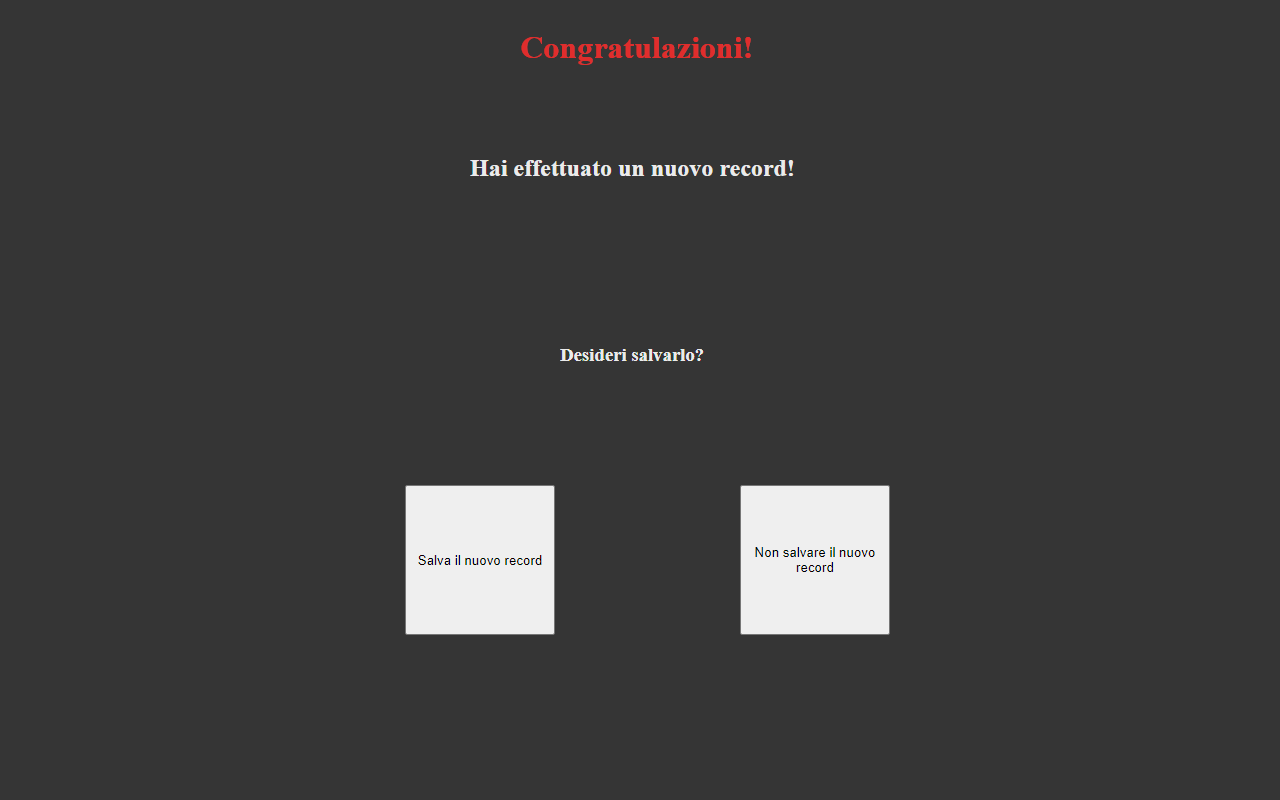
\includegraphics[width=340pt]{schermataNuovoRecord.png}
    \caption{Schermata di avviso per un nuovo record}
    \label{fig:schermataNuovoRecord}
\end{figure}
\subsection{Pagina di inserimento nome-stile arcade}
Nel caso l'utente decidesse di salvare il record, ne viene richiesto l'inserimento del nome attraverso questa schermata.\\
Il nome viene inserito come nei vecchi cabinati arcade, ovvero selezionando tre caratteri da una lista di caratteri. Per la selezione, vengono utilizzati gli appositi pulsanti, situati sopra e sotto ogni singola lettera.\\
Alla conferma, il nome viene messo sul record e salvato, e sarà dunque visibile nell'apposita schermata.
\begin{figure}[h]
    \centering
    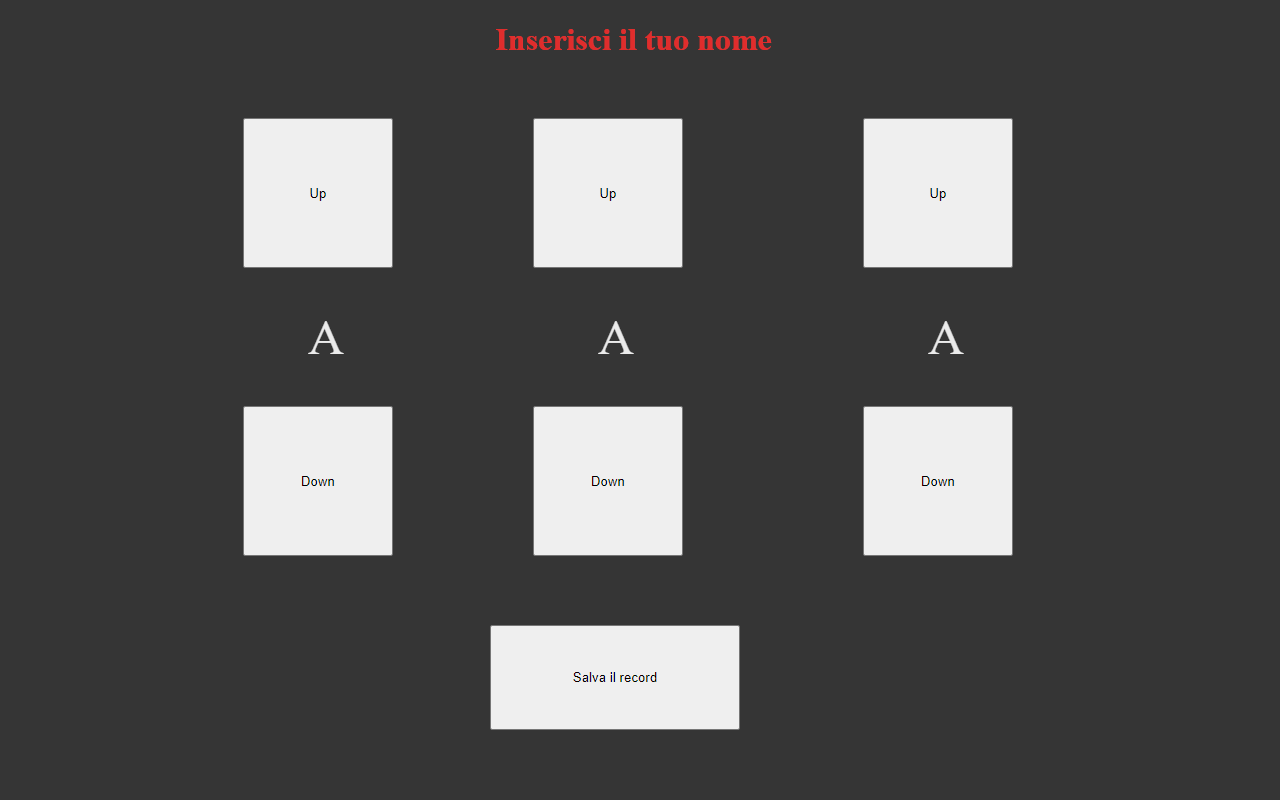
\includegraphics[width=340pt]{schermataInserimentoNome.png}
    \caption{Schermata per l'inserimento del nome}
    \label{fig:schermataInserimentoNome}
\end{figure}
\subsubsection{Inattività nell'inserimento di un nuovo nome}
Per quanto accade durante un'eventuale inattività, si rimanda alla sezione di \hyperref[sec:inactivity]{Gestione dell'inattività}
\newpage
\section{Gestione dell'inattività}
\label{sec:inactivity}
L'applicazione, se non rileva alcun input per 10 secondi, fa partire un timer di inattività della durata massima di 4 minuti. Tale timer si azzera se durante questo lasso di tempo riceve un input.\\
Nel caso scada il tempo, il sistema chiude l'attività in esecuzione (gioco o salvataggio del record) e ritorna alla schermata principale.\\
Tale azione comporta la perdita di un eventuale record effettuato, in quanto l'attività precedentemente in esecuzione viene chiusa forzatamente.